\section{绪论}

\subsubsection{同源器官和同工器官}

同源器官指的是内在的、实质性的相似,表明在进化上的共同起源。它们也许在表面上有很大不同,功能也未必相似,但是在基本结构、胚胎发生的来源等方面是相同或相似的。如鸟的翅、海豹的前鳍足和猫的前肢。比较解剖学特别注重对同源器官的探讨。

同功器官只是一般的功能相似,是表面上的相似。如鱼的鳃和陆生动物的肺,都行使呼吸功能,却是非同源的。

\section{脊索动物门总论}

\subsection{脊索动物门的共同特征}

脊索动物的共同特征是具脊索、背神经管和鳃裂(\autoref{fig:comparision_main_feature})。

\begin{wrapfigure}{r}{0.3\textwidth}
	\centering
	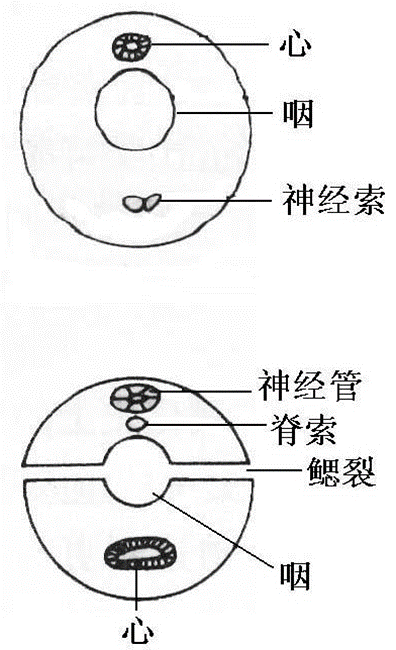
\includegraphics[width=\linewidth]{Pics/脊索动物和无脊椎动物横截面}
	\caption{无脊椎动物(上)与脊椎动物(下)特征比较}
	\label{fig:comparision_main_feature}
\end{wrapfigure}

\begin{description}
	\item[脊索] 纵贯身体背部的弹性棒状支持结构,位于消化管背面、神经管腹面。弹性和硬度来源于脊索内具有液泡的细胞,脊索外面包有坚韧的脊索鞘。
	\item[背神经管] 胚胎背中部的外胚层下陷卷起形成的,内部中空。脊椎动物的神经管前部膨大形成脑,其余部分成为脊髓。空腔仍然保留,形成脑部的脑室和脊髓处的中央管。作为对比,某些具有中枢神经的无脊椎动物的腹神经是实心的索状。
	\item[咽囊、鳃裂] 咽囊是内胚层向外膨出形成的囊状结构。与此同时,外胚层向内凹陷形成咽沟,二者最终打通中胚层形成鳃裂。水生脊索动物的咽囊打通形成鳃裂,陆生的则具有咽囊,但仅在胚胎期或幼体期打通成鳃裂,成体时咽囊消失或转变为其他结构(\autoref{tab:pharyngeal_pouch_development})。有些人具有颈裂,这是鳃裂未关闭的痕迹。
\end{description}

脊索动物还有一些次要的特征:
\begin{description}
	\item[心脏] 总是位于腹面。(注意文昌鱼没有心脏)
	\item[肛后尾] 意思是位于肛门后方的尾。
	\item[中胚层来源的内骨骼] 中胚层生骨节形成骨骼,表面有肌肉附着。
	\item[咽下腺] 位于咽的腹面,在低等脊索动物中称为内柱或咽下腺,脊椎动物中称为甲状腺。显然二者是同源结构。
\end{description}

\subsection{起源和演化}

现在认为,脊索动物和棘皮动物有共同祖先,证据如下:
\begin{itemize}
	\item 二者同属于后口动物,以体腔囊法形成体腔;
	\item 棘皮动物和半索动物幼虫相似;
	\item 棘皮动物和半索动物肌肉中都兼含有肌酸(脊索动物)和精氨酸(无脊椎动物)。
\end{itemize}

脊索动物进化的里程碑:脊椎骨的出现$\longrightarrow$上下颌的出现$\longrightarrow$水生到陆生$\longrightarrow$羊膜卵的出现$\longrightarrow$恒温动物的出现。

\begin{table}[h]
	\centering
	\begin{tabularx}{\textwidth}{|c|C|C|C|C|C|}
		\hline
		& 脊椎骨 & 有无颌 & 水或陆生 & 羊膜 & 体温 \\ \hline
		尾索动物 & \multirow{2}{*}{无} & \multirow{3}{*}{无颌类} & \multirow{5}{*}{水生} & \multirow{6}{*}{无羊膜类} & \multirow{7}{*}{变温} \\ \cline{1-1}
		头索动物 &  &  &  &  &  \\ \cline{1-2}
		圆口纲 & 雏形 &  &  &  &  \\ \cline{1-3}
		软骨鱼 & \multirow{6}{*}{有} & \multirow{6}{*}{颌口类} &  &  &  \\ \cline{1-1}
		硬骨鱼 &  &  &  &  &  \\ \cline{1-1} \cline{4-4}
		两栖 &  &  & 过渡 &  &  \\ \cline{1-1} \cline{4-5}
		爬行 &  &  & \multirow{3}{*}{陆生} & \multirow{3}{*}{羊膜类} &  \\ \cline{1-1} \cline{6-6}
		鸟 &  &  &  &  & \multirow{2}{*}{恒温} \\ \cline{1-1}
		哺乳 &  &  &  &  &  \\ \hline
	\end{tabularx}
	\caption{脊索动物进化里程碑}
	\label{tab:revolutional_milestone}
\end{table}

\section{体腔和系膜}

\subsection{体腔}

体腔是中胚层侧板(下节)中的空腔。

鱼类、两栖类、爬行类的体腔分为心包腔和胸腹腔;鳄、鸟类、哺乳类的体腔分为心包腔、2个胸腔、腹腔。鸟类以斜隔、哺乳类以横隔分开胸腔和腹腔。

\subsection{系膜}

下节中胚层中,外侧(体壁中胚层)与体壁相贴形成腹膜;内侧(脏壁中胚层)包围肠管,形成脏膜(浆膜)。脏膜包括背面的背系膜和腹面的腹系膜。

脊椎动物中,腹系膜大部分退化,背系膜大部分保存。残留的腹系膜只有胃干十二指肠韧带。


\section{皮肤及其衍生物}


\section{骨骼系统}

骨骼依照其作用和形态分为\autoref{tab:varied_bones}所示的几类。

\begin{table}[htbp]
	\centering
	\begin{tabularx}{\textwidth}{|c|X|X|X|}
		\hline
		\textbf{类别} & \multicolumn{1}{c|}{\textbf{形态特点}} & \multicolumn{1}{c|}{\textbf{功能}} & \multicolumn{1}{c|}{\textbf{举例}} \\ \hline
		长骨 & 管状,两端具骨垢 & 支持、杠杆 & 四肢骨、肋骨 \\ \hline
		短骨 & 方形或圆形小骨 & 支持、杠杆、分压 & 椎骨、籽骨 \\ \hline
		扁骨 & 扁平 & 保护、附着肌肉 & 头盖骨、肩胛骨 \\ \hline
		不规则骨 & 不规则 &  &  \\ \hline
	\end{tabularx}
	\caption{骨的类型}
	\label{tab:varied_bones}
\end{table}

骨垢与长骨的骨干之间有垢软骨连接,它的生长和骨化使长骨增长。垢软骨完全骨化后,长骨就无法再变长。这就是小孩才能长高的原因。

脊椎动物的骨骼分为中轴骨和附肢骨(\autoref{fig:bone_types})。

\begin{figure}[htbp]
	\centering
	\begin{forest}
		forest scheme
		[骨骼
			[中轴骨
				[头骨]
				[脊柱]]
			[附肢骨
				[带骨
					[肩带]
					[腰带]]
				[附肢骨]]]
	\end{forest}
	\caption{脊椎动物骨骼分类}
	\label{fig:bone_types}
\end{figure}

\subsection{脊柱和肋骨、胸骨}

\subsubsection{脊柱}

\subsubsection{肋骨}

肋骨近端与脊椎骨相连,远端游离;或经肋软骨与胸骨相连,这样构成胸廓。

\paragraph{背肋与腹肋}

肋骨分为背肋和腹肋两类:(\autoref{tab:背肋和腹肋的比较})

\begin{table}[htbp]
	\centering
	\begin{tabularx}{\textwidth}{|c|c|c|C|}
		\hline
		肋骨 & 发生位置 & 别称 & 举例 \\ \hline
		背肋 & 肌隔与水平生骨隔交线 & 肌间肋 & 鲨鱼、陆生脊椎动物 \\ \hline
		腹肋 & 肌隔与腹生骨隔交线 & 腹膜下肋 & 硬骨鱼 \\ \hline
	\end{tabularx}
	\caption{背肋和腹肋的比较}
	\label{tab:背肋和腹肋的比较}
\end{table}

少数种类(如多鳍鱼)兼具背肋和腹肋。

背肋和腹肋仅是对于发育过程中的位置而言,成体动物的肋骨都伸向腹面。

最初形成的肋骨为软骨,之后部分或完全骨化成硬骨。陆生脊椎动物的肋骨在与胸骨相连的那段不骨化。

每一椎骨一般都有一对肋骨,但是通常只有胸部的发达,其余部分的退化。

\paragraph{肋骨比较}


\subsection{头骨}

脊椎动物的头骨(亦称颅骨)由软颅、咽颅、膜颅组成。

\subsubsection{咽颅}

\begin{table}[htbp]
	\centering
	\begin{tabularx}{\textwidth}{|c|C|c|c|c|c|}
		\hline
		& 软骨鱼 & 硬骨鱼 & 两栖 & 爬行、鸟类 & 哺乳 \\ \hline
		第一咽弓 & 腭方软骨(上颌) & 方骨 & 方骨 & 方骨 & 砧骨 \\ \cline{2-6}
		(颌弓) & 麦氏软骨(下颌) & 关节骨 & 关节骨 & 关节骨 & 锤骨 \\ \hline
		& 舌颌软骨 & 舌颌骨 & 耳柱骨 & 耳柱骨 & 蹬骨 \\ \cline{2-6}
		第二咽弓 &  & 续骨 &  &  &  \\ \cline{2-6}
		(舌弓) & 角舌软骨 & 舌骨 & 舌骨 & 舌骨 & 舌骨 \\ \cline{2-6}
		& 基舌软骨 & 舌骨 & 舌骨 & 舌骨 & 舌骨 \\ \hline
		第三咽弓 & \multirow{2}{*}{鳃弓} & \multirow{2}{*}{鳃弓} & \multirow{2}{*}{舌骨} & \multirow{2}{*}{舌骨} & \multirow{2}{*}{舌骨} \\
		(第一鳃弓) &  &  &  &  &  \\ \hline
		第四咽弓 & \multirow{2}{*}{鳃弓} & \multirow{2}{*}{鳃弓} & \multirow{2}{*}{舌骨} & \multirow{2}{*}{舌骨} & \multirow{2}{*}{甲状软骨} \\
		(第二鳃弓) &  &  &  &  &  \\ \hline
		第五咽弓 & \multirow{2}{*}{鳃弓} & \multirow{2}{*}{鳃弓} & \multirow{2}{*}{喉头软骨} & \multirow{2}{*}{喉头软骨} & \multirow{2}{*}{喉头软骨} \\
		(第三鳃弓) &  &  &  &  &  \\ \hline
		第六咽弓 & \multirow{2}{*}{鳃弓} & \multirow{2}{*}{鳃弓} & \multirow{2}{*}{消失} & \multirow{2}{*}{消失} & \multirow{2}{*}{消失} \\
		(第四鳃弓) &  &  &  &  &  \\ \hline
		第七咽弓 & \multirow{2}{*}{鳃弓} & \multirow{2}{*}{鳃弓} & \multirow{2}{*}{消失} & \multirow{2}{*}{消失} & \multirow{2}{*}{消失} \\
		(第五鳃弓) &  &  &  &  &  \\ \hline
	\end{tabularx}
	\caption{脊椎动物咽颅的比较}
	\label{tab:vertebrate_pharyngeal_skull_comparison}
\end{table}

\subsubsection{陆生脊椎动物的四肢}

\begin{table}[h]
	\centering
	\begin{tabularx}{\textwidth}{|>{\centering\arraybackslash}m{6em}|X|X|}
		\hline
		\multicolumn{1}{|c|}{\textbf{四肢着地方式}} & \multicolumn{1}{c|}{\textbf{特点}} & \multicolumn{1}{c|}{\textbf{代表动物}} \\ \hline
		跖行性 & 以全部脚掌着地,较原始 & 猿猴、人 \\ \hline
		趾行性 & 只有脚趾着地 & 猫、犬 \\ \hline
		蹄行性 & 以蹄(趾尖)着地,适于奔跑 & 奇蹄目、偶蹄目 \\ \hline
	\end{tabularx}
	\caption{哺乳动物行走时四肢着地部位}
	\label{tab:mammal_walk}
\end{table}







\section{肌肉系统}

\subsection{概述}

\subsubsection{肌肉的功能与结构}

肌肉是许多层次的束状结构与包膜“套娃”形成的。如下:

\begin{enumerate}
	\item 单根肌纤维外包有肌内膜;
	\item 多根肌纤维成肌纤维束,外包肌束膜;
	\item 多根肌纤维束形成肌肉,肌肉外包肌外膜。
\end{enumerate}

肌纤维有红、白之分,使得肌肉有红肌(大腿肌)、白肌(鸟的胸肌)之分。(\autoref{tab:red_white_muscle})

\begin{table}[htbp]
	\centering
	\begin{tabularx}{\textwidth}{|C|C|c|c|c|c|C|c|}
		\hline
		\textbf{肌纤维} & \textbf{肌红蛋白} & \textbf{直径} & \textbf{血管} & \textbf{线粒体} & \textbf{收缩力} & \textbf{反应} & \textbf{疲劳} \\ \hline
		红肌纤维 & 多 & 细 & 多 & 多 & 小 & 慢、持久 & 不易 \\ \hline
		白肌纤维 & 少 & 粗 & 少 & 少 & 大 & 快、短暂 & 易 \\ \hline
	\end{tabularx}
	\caption{红肌纤维和白肌纤维的比较}
	\label{tab:red_white_muscle}
\end{table}


\subsubsection{肌肉的种类}

见\autoref{fig:class_muscles}。

\begin{figure}[htbp]
	\centering
	\begin{forest}
		forest scheme
		[肌肉
			[骨骼肌
				[体节肌
					[躯干肌和尾肌
						[轴上肌]
						[轴下肌]]
					[鳃下肌和舌肌]
					[外生眼球肌]
					[附肢肌
						[内生肌]
						[外生肌]]]
				[鳃节肌
					[颌弓肌]
					[舌弓肌]
					[鳃弓肌]]
				[皮肤肌]
				]
				[心肌]
				[平滑肌]]
	\end{forest}
	\caption{脊椎动物肌肉的分类}
	\label{fig:class_muscles}
\end{figure}

\subsubsection{肌肉的胚胎发生}

\begin{itemize}
	\item 生肌节——体节肌;
	\item 脏壁中胚层——平滑肌、心肌、鳃节肌;
	\item 体节肌和鳃节肌分离——皮肤肌。
\end{itemize}

\subsection{体节肌}

\subsubsection{躯干肌}

\subsubsection{鳃下肌、舌肌}

\subsubsection{外生眼球肌}

\section{消化系统}

消化系统包括消化道和消化腺,皆由胚胎期的原肠分化而来。消化道各胚层来源如下:

\begin{itemize}
	\item 内胚层:大部分原肠;
	\item 上节中胚层:消化道外壁的结缔组织;
	\item 外胚层:原肠两端的原口、原肛。
\end{itemize}

原肠管在成体动物中分化为整个消化道及泄殖腔。

原肠衍生物有:垂体前叶(实际上来源于体壁外胚层)、咽囊、甲状腺、\xpinyin*{鳔}、肺、肝、胰、卵黄囊、尿囊等。

\subsection{肠}

从内到外,消化管管壁分为黏膜、黏膜下层、肌层、浆膜,其中只有黏膜来源于内胚层,其他三者来源于中胚层。

\subsection{牙齿}


\begin{table}[h]
	\centering
	\begin{tabularx}{\textwidth}{|c|CCCC|C|C|}
		\hline
		& \multicolumn{1}{C|}{软骨鱼} & \multicolumn{1}{C|}{硬骨鱼} & \multicolumn{1}{C|}{两栖} & 爬行 & 鸟 & 哺乳 \\ \hline
		着生方式 & \multicolumn{1}{c|}{结缔组织} & \multicolumn{2}{c|}{端生} & 三种兼备 & \multirow{3}{*}{无牙齿} & 槽生 \\ \cline{1-5} \cline{7-7}
		出齿类型 & \multicolumn{4}{c|}{多出} &  & 再出 \\ \cline{1-5} \cline{7-7}
		牙齿形状 & \multicolumn{4}{c|}{同形} &  & 异形 \\ \hline
	\end{tabularx}
	\caption{脊椎动物齿的比较}
	\label{tab:vertebrate_tooth_comparison}
\end{table}

爬行动物的牙齿着生方式上具有多样性:

\begin{itemize}
	\item 端生齿:古代蛇;
	\item 侧生齿:蛇、蜥蜴;
	\item 槽生齿:鳄。
\end{itemize}

毒蛇上颌的牙齿一般有2个变为沟牙或管牙,是空心的。毒牙后常有后备齿,前面的毒牙失掉后就递补上去。闭口时毒牙倒卧,咬噬时肌肉收缩,毒牙竖立。

蜥蜴及一些蛇类的胚胎,有卵齿,用于啄破卵壳,孵出后不久即脱落。

另外,楔齿蜥、龟、鳄在胚胎的吻上有角质齿,功能类似,但不与牙齿同源,它是表皮衍生物。

哺乳动物的牙齿有门齿、犬齿、前臼齿、臼齿的分化。这些牙齿的特征随食性而变化(\autoref{tab:tooth_differ})。

\begin{table}[h]
	\centering
	\begin{NiceTabularX}{\textwidth}{|c|c|c|C|}
		\hline
		食性 & 门齿 & 犬齿 & 前臼齿、臼齿 \\ \hline
		食虫类 & 尖 & 不发达 & 臼齿三尖齿,齿尖呈“W”形 \\ \hline
		肉食类 & 小 & 发达 & 裂齿\tabularnote{裂齿是上颌最后一颗前臼齿与下颌第一颗臼齿形成的交错结构。} \\ \hline
		草食类 &  & 缺失,有齿虚位 & 臼齿新月形,齿冠高 \\ \hline
		杂食类 &  &  & 臼齿丘型齿 \\ \hline
	\end{NiceTabularX}
	\caption{不同食性动物的牙齿分化}
	\label{tab:tooth_differ}
\end{table}

臼齿具有显著的形态差异。臼齿的结构既可作为分类依据,又可鉴定年龄。象具有特征性的\sy{脊形齿}(\autoref{fig:大象的臼齿})。

\begin{figure}[htbp]
	\centering
	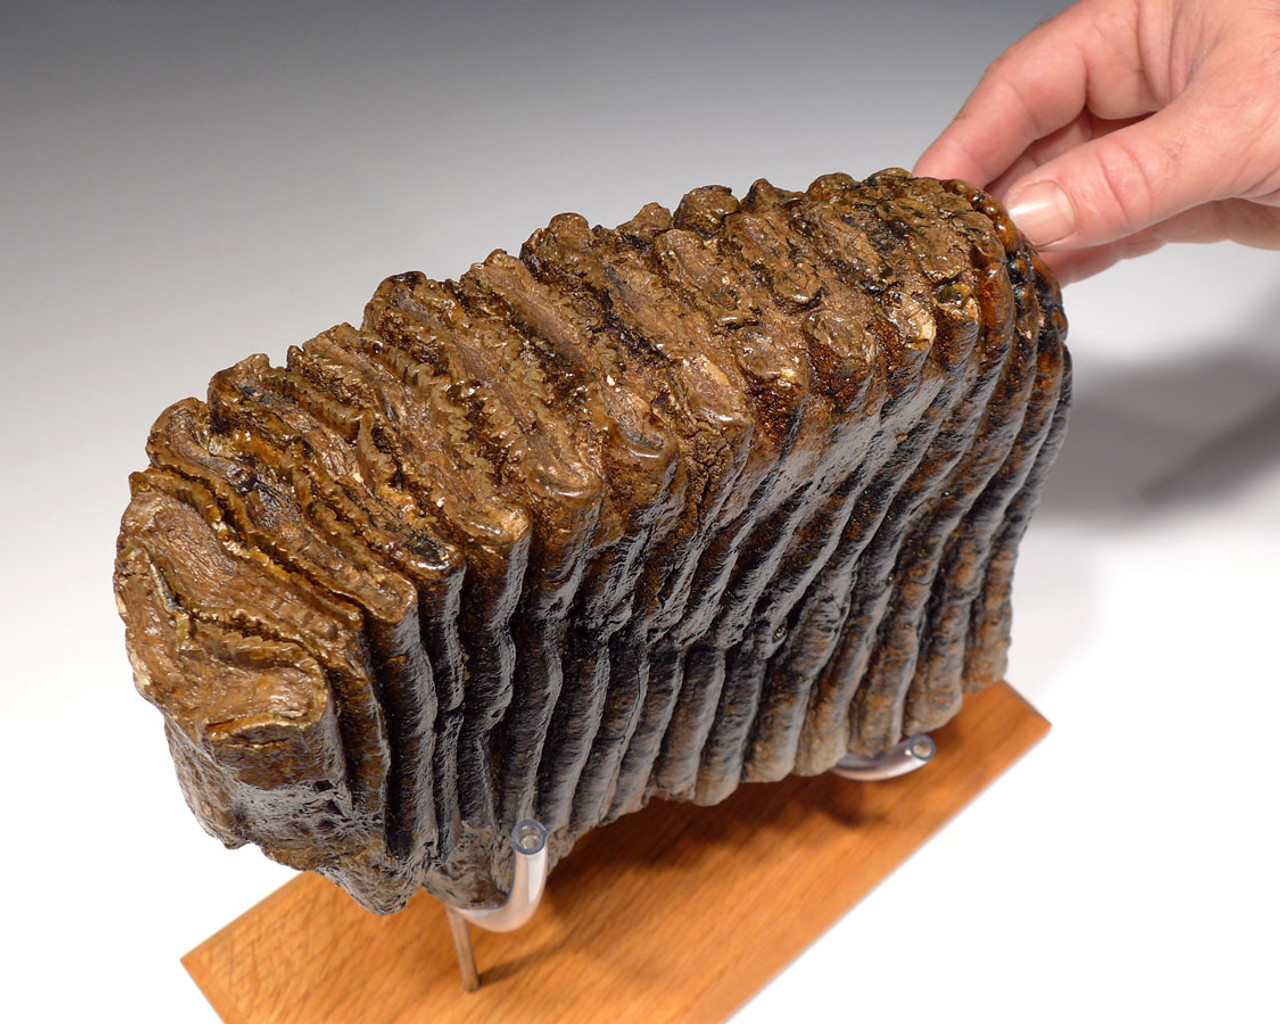
\includegraphics[width=0.4\linewidth]{大象的臼齿}
	\caption{大象的臼齿}
	\label{fig:大象的臼齿}
\end{figure}


\subsection{舌}

不同动物舌的特点:

\begin{itemize}
	\item 文昌鱼无舌;
	\item 无颌类(圆口纲)有舌,适于吸食血肉;
	\item 鱼类有舌,但没有舌内肌,只可稍作前后挪动;
	\item 无尾两栖类开始有舌内肌,能自由伸缩;
	\item 爬行类中有鳞类的舌活动性更大,如蛇和一些蜥蜴的舌可以伸出很远、避役(变色龙)的舌成为特殊的捕食器;
	\item 鸟类的舌表面覆有角质上皮,硬;
	\item 哺乳动物有发达的肌肉质的舌。舌表面有4种乳头:丝状乳头、蕈状乳头、轮廓乳头、叶状乳头(\autoref{tab:mammal_tongue})。
\end{itemize}



\begin{table}[htbp]
	\centering
	\begin{tabularx}{\textwidth}{|c|c|C|C|c|}
		\hline
		\textbf{舌乳头} & \textbf{数量} & \textbf{形态} & \textbf{分布} & \textbf{味觉} \\ \hline
		丝状乳头 & 最多 & 绒毛状 & 密布舌背面 & 否 \\ \hline
		蕈状乳头 & 较少 & 蕈状,顶端呈圆形 & 舌尖较多 & 是 \\ \hline
		轮廓乳头 & 一对 & 圆形 & 舌根 & 是 \\ \hline
		叶状乳头 & 一对 & 椭圆形,表面有平行皱褶 & 轮廓乳头外侧前缘 & 是 \\ \hline
	\end{tabularx}
	\caption{哺乳动物的舌乳头}
	\label{tab:mammal_tongue}
\end{table}

\subsection{口腺}

\begin{table}[htbp]
	\centering
	\begin{tabularx}{\textwidth}{|c|X|c|}
		\hline
		\textbf{类群} & \multicolumn{1}{c|}{\textbf{口腺情况}} & \textbf{有无消化酶} \\ \hline
		无颌类 & 有,可使寄主血液不凝 & 无 \\ \hline
		鱼类 & 无口腺 & 无 \\ \hline
		两栖类 & 颌间腺 & 无 \\ \hline
		爬行类 & 唇腺、腭腺、舌腺、舌下腺,毒腺是变态的口腺 & 无 \\ \hline
		鸟类 & 食谷的发达 & 无\footnotemark \\ \hline
		哺乳类 & 耳下腺、颌下腺、舌下腺,兔还有眶下腺 & 有 \\ \hline
	\end{tabularx}
	\caption{脊椎动物口腺比较}
	\label{tab:oral_gland}
\end{table}

\subsection{咽}

鱼类胚胎早期形成6对咽囊,随后打通形成鳃裂。鳃裂之间为鳃隔,其上着生鳃丝形成鱼鳃。

陆栖脊椎动物虽用肺呼吸,胚胎期仍然形成5对咽囊,以后形成其他结构(\autoref{tab:pharyngeal_pouch_development})

\begin{table}[htbp]
	\centering
	\begin{tabularx}{\textwidth}{|c|X|}
		\hline
		咽囊 & \multicolumn{1}{c|}{发育形成的器官} \\ \hline
		第一对 & 鲨鱼的喷水孔、中耳鼓室、咽鼓管 \\ \hline
		第二对 & 第一对鳃裂、腭扁桃体 \\ \hline
		第三对 & 胸腺、下一对甲状旁腺 \\ \hline
		第四对 & 上一对甲状旁腺 \\ \hline
		第五对 & 后鳃体 \\ \hline
	\end{tabularx}
	\caption{咽囊的发育}
	\label{tab:pharyngeal_pouch_development}
\end{table}

成体咽部是食物进入食道、呼吸介质进入鳃或肺的共同道路。

\begin{itemize}
	\item 鱼类,水与食物共同入口,水由鳃裂流出,同时进行气体交换,食物进入食道;
	\item 两栖类,内鼻孔出现,空气就从鼻孔经过口入肺。两栖类口腔和咽无分界,称为口咽腔;
	\item 爬行类,口腔和咽有明显分界;
	\item 哺乳类,内鼻孔后移,形成软腭,空气可直接经咽入肺而不经过口。
\end{itemize}

哺乳类中,空气通路和食物通路在咽部形成咽交叉,使得我们满嘴食物依然能呼吸。食物经过咽的时候,会厌软骨盖住喉门,防止食物误入气管。

\subsection{食道与胃}

\begin{wrapfigure}{r}{0.3\textwidth}
	\centering
	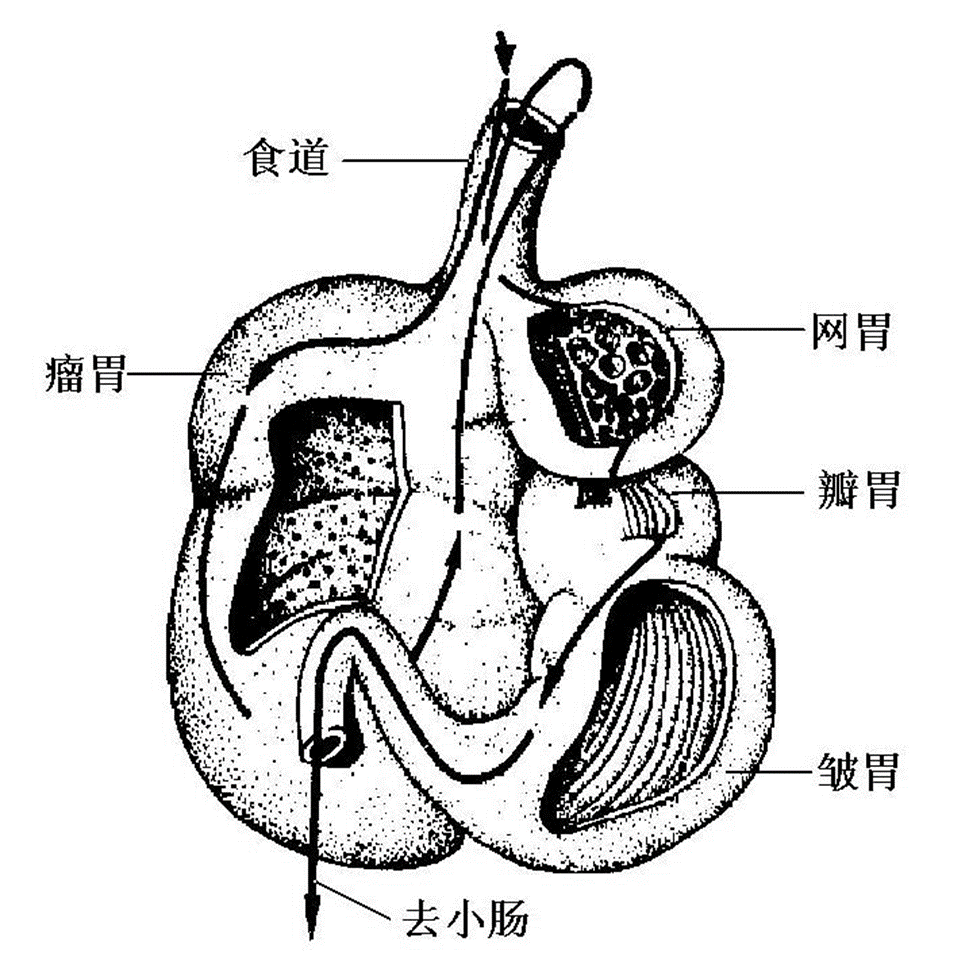
\includegraphics[width=\linewidth]{Pics/反刍胃}
	\caption{反刍动物的胃}
	\label{fig:cow_stomach}
\end{wrapfigure}

文昌鱼和无颌类尚无食道和胃的分化。

鸟类的食道在中部扩大形成嗦囊,临时储存和软化食物。鸽的嗦囊壁还能分泌“鸽乳”以哺幼。吸血蝠的食道极其细,只能通过血液。

从鱼类开始就出现了胃,与上下颌出现、适于摄取大型食物相关。

胚胎时期的胃和低等脊椎动物的胃是一直管;多数脊椎动物的胃呈“J”或“U”型的明显膨大。胃以\xpinyin{贲}{ben1}门与食道相连,以幽门与十二指肠相连。鸟类的胃有腺胃和肌胃(砂囊)的分化。腺胃分泌大量消化液,肌胃负责研磨食物。

食草动物反刍类的胃(\autoref{fig:cow_stomach})属于多室胃,如牛羊。瘤胃、网胃、瓣胃、皱胃中,只有皱胃是胃的本体,只有它才分泌消化液。

食物$\longrightarrow$口腔$\longrightarrow$瘤胃$\longrightarrow$网胃$\longrightarrow$反刍至口腔$\longrightarrow$瓣胃$\longrightarrow$皱胃

骆驼的胃缺少瓣胃。骆驼的瘤胃周围分生出许多储水用的小囊。

\subsection{肠}

肠的复杂程度和进化水平、食性都有关系。

\begin{itemize}
	\item 文昌鱼、无颌类、鱼类尚无肠的分化,就是一条管;
	\item 两栖类有小肠和大肠的分化,但大肠很短;
	\item 爬行类第一次出现盲肠;
	\item 鸟类有一对盲肠,草食性和杂食性鸟类中特别发达;
	\item 哺乳类小肠分化成十二指肠、回肠、空肠,大肠分化成盲肠、结肠、直肠;草食性哺乳动物的盲肠很发达,它们的肠总长度也是最长的。
\end{itemize}

增加肠的消化吸收面积有以下几种方式:

\begin{description}
	\item[盲沟] 七鳃鳗具有。
	\item[螺旋瓣肠] 较原始。鲨鱼、银鲛、非洲肺鱼、鲟鱼等。
	\item[幽门盲囊] 有些硬骨鱼具有,但所有硬骨鱼都没有螺旋瓣肠。
	\item[增加肠的长度] 多数脊椎动物。植食性的肠较长,肉食性较短。
	\item[突起] 如小肠绒毛。
\end{description}

\section{呼吸系统}

\subsubsection{鳃}



\subsubsection{鳔和肺}

\section{排泄系统}

\subsection{肾脏}

\begin{table}[htbp]
	\centering
	\begin{NiceTabularX}{\textwidth}{cXXX}[hvlines]
		& \Block[c]{1-1}{前肾} & \Block[c]{1-1}{中肾、后位肾} & \Block[c]{1-1}{后肾} \\
		\Block{2-1}{系统发生} & 无羊膜类胚胎期具有泌尿功能 & 后位肾——无羊膜类成体肾脏 &  \\
		& 羊膜类胚胎期经历此阶段 & 中肾——羊膜类胚胎期肾脏 & 羊膜类成体肾脏 \\
		个体发生 & 胚胎期最早出现 & 较晚出现 & 羊膜类最后出现 \\
		\Block[v-center]{1-1}{位置} & 位于体腔前部 & 后位肾——位于体腔中、后部;中肾——位于体腔中部 & 体腔后部 \\
		\Block{3-1}{结构特点} & 前肾小管数目少 & 中肾小管数目较多、出现肾小体 & 后肾小管数目极多 \\
		& 肾孔开口于体腔 & 肾孔从有到无 & 无肾孔 \\
		& 体腔联系 & 体腔联系从有到无、建立血管联系 & 仅有血管联系 \\
		\Block[v-center]{1-1}{管道} & 前肾管——胚胎期的输尿管 & 中肾管 & 后肾管——羊膜类成体的输尿管
	\end{NiceTabularX}

	\mbox{}\vspace{1em}

	\begin{NiceTabularX}{\textwidth}{cCCCC}[hvlines]
		\Block{2-1}{中肾管}& \Block{1-2}{无羊膜类} &  & \Block{1-2}{羊膜类} &  \\
		& 雄 & 雌 & 雄 & 雌 \\
		吴氏管 & 输尿、输精 & 输尿 & 输精 & 退化 \\
		牟勒氏管 & 退化 & 输卵 & 退化 & 输卵
	\end{NiceTabularX}

	\caption{脊椎动物肾脏类型比较}
	\label{tab:kidney_compare}
\end{table}

脊椎动物肾脏的比较见\autoref{tab:kidney_compare}。

需要注意一下一些名词的别称,以防考试时不认识:
\begin{description}
	\item[吴氏管] 又称中肾管。
	\item[牟勒氏管] 又称米氏管。
\end{description}

各种鱼的排泄情况如\autoref{tab:fish_osmotic_regulation}所示:

体液浓度:软骨鱼$>$海水$>$硬骨鱼$>$淡水

\begin{table}[htbp]
	\centering
	\begin{tabularx}{\textwidth}{|C|c|C|C|c|c|c|}
		\hline
		鱼类 & 肾小球 & 排盐部位 & 体液浓度 & 喝水 & 排泄物 & 尿量 \\ \hline
		软骨鱼 & 较多 & 直肠腺 & 高于海水 & 否 & 尿素 &  \\ \hline
		淡水硬骨鱼 & 多 & 鳃上泌氯腺\footnotemark & 高于淡水 & 否 & 铵盐 & 多 \\ \hline
		海水硬骨鱼 & 少 & 鳃上泌氯腺 & 比海水略低 & 是 & 铵盐 & 少 \\ \hline
	\end{tabularx}
	\caption{鱼类渗透压调节}
	\label{tab:fish_osmotic_regulation}
\end{table}
\footnotetext{淡水硬骨鱼的泌氯腺是吸收盐分用的。}

\subsection{输尿管、膀胱、排泄产物}

\subsubsection{输尿管}

\begin{itemize}
	\item 七鳃鳗的中肾管即为输尿管,和生殖无关,七鳃鳗不具任何生殖管道;
	\item 雄性鲨类另外形成副肾管排尿,中肾管用于输精;
	\item 硬骨鱼的中肾管仅用作输尿,生殖腺自身形成管道输精,这是很特殊的;
\end{itemize}

\subsubsection{泄殖腔与泄殖窦}

\begin{table}[htbp]
	\centering
	\begin{NiceTabularX}{\textwidth}{cXX}[hvlines]
		& \Block[c]{1-1}{泄殖腔} & \Block[c]{1-1}{泄殖窦} \\
		\Block[v-center]{1-1}{结构} & 消化管、输尿管、生殖管末端共同汇合处 & 仅泌尿系统与生殖系统末端汇合处,消化道通过肛门单独开口 \\
		\Block[v-center]{1-1}{开口数} & 三个开口(消化、排泄、生殖)合并为一个泄殖腔孔 & 两个开口(排泄、生殖)合并为泄殖孔,消化道通过肛门独立开口 \\
		\Block[v-center]{1-1}{功能} & 同时排出粪便、尿液和生殖细胞(如卵或精子)& 仅排出尿液和生殖细胞,粪便通过肛门单独排出 \\
		\Block[v-center]{1-1}{动物} & 两栖类、软骨鱼、爬行类、鸟类及单孔类 & 见于圆口类、硬骨鱼、全头类(如银鲛)及有胎盘哺乳动物
	\end{NiceTabularX}
	\caption{泄殖腔与泄殖窦的比较}
	\label{tab:ComparisonOfCloacaAndUrogenitalSinus}
\end{table}

\subsubsection{膀胱}

圆口类、软骨鱼、少数硬骨鱼(如比目鱼)、部分爬行类(蛇、鳄、一部分蜥蜴)、除鸵鸟外所有鸟类全无膀胱。

膀胱可分三种类型:(\autoref{tab:bladder})

\begin{table}[htbp]
	\centering
	\begin{tabularx}{\textwidth}{|c|l|X|}
		\hline
		膀胱类型 & \multicolumn{1}{c|}{发育来源} & \multicolumn{1}{c|}{动物} \\ \hline
		导管膀胱 & 中肾管后端膨大 & 硬鳞鱼、硬骨鱼 \\ \hline
		泄殖腔膀胱 & 泄殖腔腹壁突出 & 肺鱼、两栖类、单孔类 \\ \hline
		尿囊膀胱 & 胚胎时期尿囊柄基部膨大 & 龟鳖类、楔齿蜥、一些蜥蜴、鸵鸟 \\ \hline
	\end{tabularx}
	\caption{膀胱的分类}
	\label{tab:bladder}
\end{table}

有些淡水龟鳖类还有两个副膀胱,雌性在副膀胱内储水,供产卵时润湿土壤,也可以辅助呼吸。

一些陆生四足动物的膀胱可以重吸收水分。



\section{生殖系统}

\subsection{生殖系统的来源}

生殖系统由中节中胚层生殖嵴发育而来,与排泄系统(中节中胚层生肾节发育)关系密切。生殖系统和排泄系统可合成泄殖系统。

最初,一对生殖嵴沿整个胸腹腔的长度延伸,随后,前后端都退化,只保留中间部分膨大形成生殖腺。圆口纲还保留着长形生殖腺。

\subsection{生殖腺}

\subsubsection{生殖腺的组成}

生殖腺又称性腺,在雄性即一对精巢(睾丸),在雌性即一对卵巢。尽管生殖腺都是从一对生殖嵴发育而来,但是部分脊椎动物两对生殖嵴愈合,或一侧生殖腺不分化,最后只形成一个生殖腺。

\begin{description}
	\item[生殖嵴愈合] 七鳃鳗、少数硬骨鱼;
	\item[生殖腺不分化] 盲鳗、卵胎生硬骨鱼、蜥蜴、雌鳄、大多数雌鸟、鸭嘴兽、一些蝙蝠。
\end{description}

\subsubsection{雌雄同体和性逆转}

\paragraph{雌雄同体}

雌雄同体,即同一个个体既能产生精子又能产生卵细胞,多见于圆口类,硬骨鱼和两栖类也存在。

\begin{description}
	\item[圆口纲] 盲鳗幼年,生殖腺前部是卵巢,后部是睾丸,以后何者发达则为何性别;七鳃鳗的幼体也有两性生殖腺同时存在的情况。
	\item[硬骨鱼] \xpinyin{\CJKfontspec{SimSun-ExtB}𮬜}{yi4}、海鲋的许多种终生雌雄同体、自体受精。黄鳝一开始仅有卵巢,产卵后逐渐变为精巢。黄鳝的这种变化叫\sy{性逆转}。
	\item[有尾两栖类] 蝾螈是唯一发现具雌雄同体现象的。
\end{description}

\paragraph{性逆转}

\begin{itemize}
	\item 如前所述,黄鳝具有性逆转;
	\item 无尾两栖类胚胎期精巢分为前部的毕氏器和后部的成体精巢。毕氏器在性成熟前通常消失。雄性蟾蜍的毕氏器一直保留。若摘除精巢,毕氏器将发展成为卵巢,这时在雌激素作用下,未退化的牟勒氏管发育为输卵管。
	\item 母鸡因外界因素使左侧卵巢萎缩,右侧退化的卵巢就产生雄性激素,由此可出现公鸡的第二性征。这种性逆转的鸡能产生后代\footnote{脊椎比解书中有误,敬请留意。参考资料:\href{https://d.wanfangdata.com.cn/thesis/Y1108332}{郑江霞. 人工诱导鸡性反转及鸡性别决定遗传机制研究[D]. 北京:中国农业大学,2006. DOI:10.7666/d.y1108332.}}。
\end{itemize}

\subsubsection{精巢的系统发生}

\begin{description}
	\item[七鳃鳗] 成体具单个精巢,无生殖管道。
	\item[软骨鱼] 具一对精巢,位于体腔前部。右侧精巢常常大于左侧的。
	\item[硬骨鱼] 具一对精巢,发育阶段可分为6期:

	\begin{enumerate}[label=\Roman*]
		\item 性腺未发育,可见分散精原细胞;
		\item 精巢呈细带状,血管不显著;
		\item 精巢膨大为圆柱状、白色,血管发达,出现初级精母细胞;
		\item 精巢乳白色,精细管中出现初级、次级精母细胞、精细胞、精子;
		\item 充分成熟,轻压鱼腹,可流出白色精液;
		\item 生殖期已过,精巢萎缩成细带状。
	\end{enumerate}

	\item[两栖类] 精巢的形状和体形有关。如似蛇的蚓螈,精巢长条形。无尾两栖类生殖腺呈卵圆形(青蛙)或圆柱形(蟾蜍)。精巢内分为小叶,每小叶内的所有细胞处在相同发育状态。精巢内还有脂肪体,同样来源于生殖嵴,生殖季节变小。脂肪体与生殖腺的发育密切相关,摘除脂肪体后生殖腺变小。
	\item[爬行类] 一对卵圆形的精巢。精巢内有不同发育阶段的精细胞。
	\item[鸟类] 精巢大小随生殖周期变化。长日照下精巢体积增大,为繁殖做准备。
	\item[哺乳类] 精巢内部实质被分为睾丸小叶,每个小叶内含有曲细精管。曲细精管汇合形成直细精管,最后形成附睾,是精子成熟的地方。
\end{description}

\begin{figure}[htbp]
	\centering
	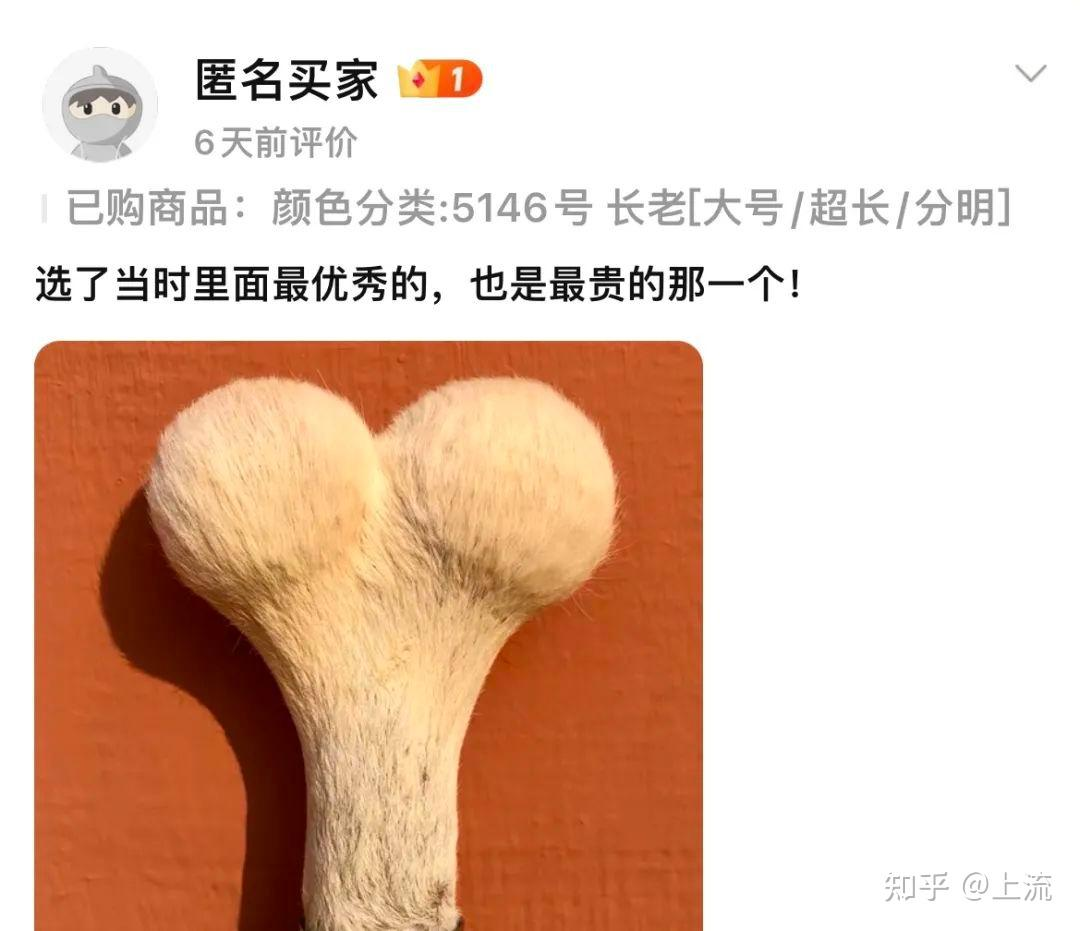
\includegraphics[width=0.7\linewidth]{Pics/袋鼠的睾丸}
	\caption{袋鼠的睾丸,被作为商品出售}
	\label{fig:ball_of_kangroo}
\end{figure}

\subsubsection{卵巢的系统发生}

\begin{description}
	\item[圆口类] 一对卵巢愈合成一个,盲鳗的左侧卵巢占优势。
	\item[软骨鱼] 卵生种类具一对卵巢,胎生种类仅右侧卵巢发育,但胎生鳐类仅左侧卵巢发育;
	\item[硬骨鱼] 大多成对、空心囊状。排卵时,卵进入卵巢腔,\zhongdian{卵巢壁延续形成输卵管}。
	\item[两栖类] 空心囊状、有很大淋巴腔隙。
	\item[爬行类] 一对中实的卵巢。
	\item[鸟类] 多数鸟类仅左侧卵巢发育,右侧退化。隼形目例外,两侧卵巢均有功能。成熟的卵巢,卵细胞突起于表面,呈葡萄状。
	\item[哺乳类] 一对中实的卵巢,有皮质和髓质之分。单孔类的卵巢仅左边发达。
\end{description}

\subsubsection{精巢下降和卵巢移位}

哺乳类胚胎期的精巢和卵巢通过一韧带连接到体腔的浅凹陷。浅凹陷发育为阴囊或大阴唇。韧带成为雄性的睾丸韧带或雌性的卵巢韧带(前部)和子宫圆韧带(后部)。

哺乳类的生殖腺本来在肾脏的前面,之后发生向后移位,即精巢下降和卵巢移位。精巢下降出腹腔,形成阴囊;卵巢虽然有移位,但不会移到骨盆之外。单孔类的卵巢不发生移位。

\paragraph{精巢下降}

哺乳类之外的动物,精巢都位于腹腔内。哺乳类的精巢位置可如下分:
\begin{description}
	\item[始终留在腹腔内,无阴囊] 单孔类、一些食虫类、多数贫齿类、一些鳍脚类(海豹、海象)、象、海牛、蹄兔、犀牛、鲸;
	\item[只在生殖期间下降到阴囊] 阴囊上有睾外提肌,是腹内斜肌的延续。如刺猬、鼹鼠、翼手类、兔、多数啮齿类、一些食肉类(水獭)、管齿类、低级灵长类、少数偶蹄类。
	\item[始终在阴囊内] 多数有袋类、一些食虫类、一些贫齿类、多数食肉类、一些鳍脚类(海狗)、奇蹄类、多数偶蹄类、灵长类。
\end{description}

一般认为精巢下降的原因是腹腔较高温影响精子发育。阴囊通过蔓状静脉丛维持比腹腔低的温度。患隐睾症的人,睾丸不下降,精巢内的曲细精管常退化。

鸟的精巢无下降现象,精巢紧贴腹气囊,通过气囊内的冷空气降温。

\subsection{雄性生殖管}

脊索动物中,精子排出体外的路径有三类:
\begin{enumerate}
	\item 无生殖管道,精子先排到围鳃腔或体腔,再由腹孔或生殖孔排出体外,最原始;
	\item 由生殖腺壁本身延续成生殖管;
	\item 借用中肾管。
\end{enumerate}

下面分别按动物类群归纳:
\begin{description}
	\item[文昌鱼、七鳃鳗] 前者精巢分节排列,后者精巢集中,但二者都没有生殖管道,属于第一类;
	\item[硬骨鱼] 属于第二种,极为少见。生殖腺壁本身延续成管道。
	\item[无尾两栖类] 属于第三种。在胚胎期中肾管和睾丸的联系就已经建立。
	\item[鲨鱼] 精巢前端发出输出管,与中肾管相连。中肾管只输精。另形成副肾管输尿。
	\item[有尾两栖类] 泥螈的中肾管输尿兼输精。蝾螈、钝口螈的中肾管只输精。
	\item[羊膜动物] 羊膜类的中肾管只输精,另有后肾管输尿。
\end{description}

\subsection{副性腺、交接器}

\subsubsection{副性腺}

哺乳动物副性腺发达,包括:精囊腺、前列腺、尿道球腺。副性腺可以维持精子活力。精液中很大部分液体都来自副性腺。

鸟类无副性腺。单孔类只有尿道球腺。

\paragraph{精囊腺}

某些啮齿类,在精囊腺内侧附有凝固腺,它最后分泌,使精液凝固,封闭阴道口,防止精液外流和二次受精。

单孔类、有袋类、食肉类、鲸缺乏精囊腺。

\paragraph{前列腺}

分泌物呈碱性,中和阴道内酸性物质。

单孔类、有袋类、贫齿类、鲸类缺少前列腺。

\paragraph{尿道球腺}

也称库伯氏腺。尿道球腺首先分泌,分泌物呈碱性,中和阴道内酸性物质。

\subsection{交接器}

\subsubsection{软骨鱼类}

体内受精。鲨鱼的交接器称为鳍脚。全头类雄性除有类似鲨鱼的一对鳍脚外,尚有一对腹前鳍脚和一额鳍于头顶部。

\subsubsection{硬骨鱼类}

大多数是体外受精的,不具交接器。行体内受精的花鳉,它的交接器称为生殖足。

\subsubsection{两栖类}

无足目全是体内受精的。如蚓螈雄性的泄殖腔甚长,可外突出作为交接器,将精液输入雌体内。无尾目的尾蟾,雄体具有一个由泄殖腔伸出的管状交接器,形似一尾巴。大多数无尾两栖类是体外受精的,雄体并无交接器。

\subsubsection{爬行类}

爬行类中除楔齿蜥缺少交接器外,其余全有。爬行类的交接器分为两种不同的形式:

\begin{description}
	\item[半阴茎] 仅见于有鳞目(蛇、蜥蜴)。
	\item[单一的阴茎] 与哺乳动物的阴茎是同源结构。
\end{description}

\subsubsection{鸟类}

鸟类大都不具交接器,仅有少数种类有交接器,如鸵鸟、鸭、鹅、天鹅。这类动物的交接器为泄殖腔腹侧壁突出的\zhongdian{螺旋状突起}。

公鸡还有残存的交接器痕迹,称阴茎乳头。残存的阴茎乳头,可以作为鉴别雌雄性的标志。

\subsubsection{哺乳类}

哺乳类中:

\begin{description}
	\item[单孔类] 具有一个小阴茎,位于泄殖腔里。
	\item[有袋类] 有袋类的阴茎已伸出体外,具有伸出和缩入的能力。龟头常分两叉,和雌体的双阴道相配合。体外具有阴囊,位于阴茎前方。
	\item[有胎盘哺乳类] 具有永久伸在体外的阴茎,称\sy{外生殖器}。有些哺乳动物,在海绵体之间的阴茎中隔处生有\sy{阴茎骨},有助于增加阴茎的坚硬度。阴茎骨存在于食虫目、啮齿、食肉目、翼手目和一些低等灵长类。阴茎骨与动物分类、生殖隔离有关。
\end{description}

\section{循环系统}

\begin{table}[htbp]
	\centering
	\begin{tabularx}{\textwidth}{|c|C|C|c|c|c|c|}
		\hline
		动脉弓 & 软骨鱼 & 硬骨鱼 & 两栖类 & 爬行类 & 鸟类 & 哺乳类 \\ \hline
		I & --- & --- & --- & --- & --- & --- \\ \hline
		II & 鳃动脉I & --- & --- & --- & --- & --- \\ \hline
		III & 鳃动脉II & 鳃动脉I & 颈动脉 & 颈动脉 & 颈动脉 & 颈动脉 \\ \hline
		IV & 鳃动脉III & 鳃动脉II & 体动脉 & 体动脉 & 体动脉 & 体动脉 \\ \hline
		V & 鳃动脉IV & 鳃动脉III & --- & --- & --- & --- \\ \hline
		VI & 鳃动脉V & 鳃动脉IV & 肺皮动脉 & 右肺动脉 & 左肺动脉 & 肺动脉 \\ \hline
	\end{tabularx}
	\caption{脊椎动物动脉弓的比较}
	\label{tab:Comparative_Aortic_Arches_Vertebrates}
\end{table}





\section{神经系统}


\section{感觉器官}

\subsection{皮肤感觉器官}

\subsection{侧线系统}

\subsection{位听器官}

\subsection{视觉器官}

\subsection{血管囊}

\subsection{化学感受器——嗅觉和味觉}

\begin{table}[h]
	\centering
	\begin{tabularx}{\textwidth}{|c|CCCCCC|}
		\hline
		& \multicolumn{1}{C|}{圆口纲} & \multicolumn{1}{C|}{鱼} & \multicolumn{1}{C|}{两栖} & \multicolumn{1}{C|}{爬行} & \multicolumn{1}{C|}{鸟} & 哺乳 \\ \hline
		鼻孔 & \multicolumn{2}{c|}{外鼻孔} & \multicolumn{4}{c|}{内鼻孔} \\ \hline
		犁鼻器 & \multicolumn{2}{c|}{无} & \multicolumn{4}{c|}{有} \\ \hline
		鼻甲骨 & \multicolumn{3}{c|}{无} & \multicolumn{3}{c|}{有} \\ \hline
		功能 & \multicolumn{2}{c|}{嗅觉} & \multicolumn{4}{c|}{嗅觉、呼吸} \\ \hline
	\end{tabularx}
	\caption{脊椎动物鼻的比较}
	\label{tab:vertebrate_nasal_comparison}
\end{table}

\section{内分泌系统}